\section{Anhang}
\label{sec:Anhang}
\subsection{Messwerte}
\begin{table}[h]
    \centering
    \caption{Messwerte der ersten Messreihe mit den globalen systematischen Messfehlern $\symup{\Delta}I = \pm \SI{0,1}{\pico\ampere}$ und $\symup{\Delta}T = \pm \SI{1}{\celsius}$.}
    \label{tab:Messung1}
    \resizebox{0.63\textwidth}{!}{%
    
    \begin{tblr}{colspec= c c c | c c c | c c c}
        \toprule
        $t\,[\si{\minute}]$ & $I\,[\si{\pico\ampere}]$ & $T\,[\si{\celsius}]$ & $t\,[\si{\minute}]$ & $I\,[\si{\pico\ampere}]$ & $T\,[\si{\celsius}]$ & $t\,[\si{\minute}]$ & $I\,[\si{\pico\ampere}]$ & $T\,[\si{\celsius}]$ \\
        \midrule
        0   &   $-0,6  $      &    $-72,0 $     &   35  &   $3,0 $        &    $-28,8$      &   69  &   $1,2 $        &    $-4,0$   \\
        1   &   $-0,675$      &    $-71,2$      &   36  &   $3,3 $        &    $-27,8$      &   70  &   $1,2 $        &    $-3,3$   \\  
        2   &   $-0,75 $      &    $-70,3$      &   37  &   $3,9 $        &    $-26,8$      &   71  &   $1,2 $        &    $-3,0$   \\      
        3   &   $-0,75 $      &    $-69,3$      &   38  &   $4,2 $        &    $-25,9$      &   72  &   $0,9 $        &    $-2,4$   \\
        4   &   $-0,75 $      &    $-68,6$      &   39  &   $4,65$        &    $-25,1$      &   73  &   $1,2 $        &    $-1,9$   \\
        5   &   $-0,6  $      &    $-67,5$      &   40  &   $5,4 $        &    $-24,2$      &   74  &   $1,2 $        &    $-1,4$   \\
        6   &   $-0,6  $      &    $-66,1$      &   41  &   $6,0 $        &    $-23,4$      &   75  &   $1,2 $        &    $-0,9$   \\
        7   &   $-0,75 $      &    $-64,0$      &   42  &   $6,3 $        &    $-22,5$      &   76  &   $1,2 $        &    $-0,4$   \\
        8   &   $-0,75 $      &    $-62,2$      &   43  &   $6,75$        &    $-21,6$      &   77  &   $1,35$        &    $0,0 $   \\      
        9   &   $-0,6  $      &    $-60,1$      &   44  &   $6,9 $        &    $-20,8$      &   78  &   $1,5 $        &    $0,9 $   \\
        10  &   $-0,75 $      &    $-58,3$      &   45  &   $7,35$        &    $-20,1$      &   79  &   $1,35$        &    $1,9 $   \\
        11  &   $-0,6  $      &    $-56,3$      &   46  &   $7,5 $        &    $-19,3$      &   80  &   $1,5 $        &    $2,8 $   \\
        12  &   $-0,6  $      &    $-54,8$      &   47  &   $7,65$        &    $-18,5$      &   81  &   $1,65$        &    $3,7 $   \\
        13  &   $-0,6  $      &    $-53,2$      &   48  &   $7,65$        &    $-17,7$      &   82  &   $1,95$        &    $4,7 $   \\
        14  &   $-0,6  $      &    $-52,0$      &   49  &   $7,5 $        &    $-17,0$      &   83  &   $2,1 $        &    $5,5 $   \\
        16  &   $-0,6  $      &    $-49,3$      &   50  &   $7,35$        &    $-16,3$      &   84  &   $2,25$        &    $6,6 $   \\
        17  &   $-0,6  $      &    $-48,2$      &   51  &   $7,2 $        &    $-15,5$      &   85  &   $2,4 $        &    $7,4 $   \\
        18  &   $-0,15 $      &    $-47,0$      &   52  &   $6,45$        &    $-14,8$      &   86  &   $2,4 $        &    $8,2 $   \\
        19  &   $0,525 $      &    $-45,8$      &   53  &   $5,85$        &    $-14,0$      &   87  &   $2,7 $        &    $9,1 $   \\
        20  &   $-0,075$      &    $-44,6$      &   54  &   $5,1 $        &    $-13,3$      &   88  &   $2,7 $        &    $10,1$   \\
        21  &   $0,0    $     &    $-43,4$      &   55  &   $4,5 $        &    $-12,6$      &   89  &   $2,7 $        &    $10,9$   \\
        22  &   $-0.15 $      &    $-42,3$      &   56  &   $3,75$        &    $-12,0$      &   90  &   $2,7 $        &    $11,7$   \\  
        23  &   $0,0    $     &    $-41,0$      &   57  &   $3,3 $        &    $-11,3$      &   91  &   $2,85$        &    $12,5$   \\  
        24  &   $0,15  $      &    $-40,0$      &   58  &   $2,85$        &    $-10,7$      &   92  &   $2,85$        &    $13,2$   \\  
        25  &   $0,15  $      &    $-38,9$      &   59  &   $2,4 $        &    $-10,0$      &   93  &   $2,85$        &    $14,0$   \\  
        26  &   $0,3   $      &    $-37,7$      &   60  &   $1,95$        &    $-9,4 $      &   94  &   $2,85$        &    $14,8$   \\
        27  &   $0,6   $      &    $-36,6$      &   61  &   $1,8 $        &    $-8,8 $      &   95  &   $2,85$        &    $15,5$   \\
        28  &   $0,75  $      &    $-35,6$      &   62  &   $1,5 $        &    $-8,1 $      &   96  &   $2,85$        &    $16,1$   \\
        29  &   $0,9   $      &    $-34,6$      &   63  &   $1,2 $        &    $-7,5 $      &   97  &   $2,85$        &    $16,9$   \\
        30  &   $1,05  $      &    $-33,5$      &   64  &   $1,2 $        &    $-7,0 $      &   98  &   $2,85$        &    $17,7$   \\
        31  &   $1,2   $      &    $-32,5$      &   65  &   $1,2 $        &    $-6,3 $      &   99  &   $2,85$        &    $18,6$   \\
        32  &   $1,8   $      &    $-31,6$      &   66  &   $0,9 $        &    $-5,8 $      &   100 &   $3,0 $        &    $19,6$   \\
        33  &   $2,1   $      &    $-30,7$      &   67  &   $0,9 $        &    $-5,0 $      &   101 &   $3,0 $        &    $20,4$   \\    
        34  &   $2,7   $      &    $-29,6$      &   68  &   $1,2 $        &    $-4,5 $      &   &       &  \\
        \bottomrule
    \end{tblr}
    }
\end{table}



\begin{table}[h]
    \centering
    \caption{Messwerte der zweiten Messreihe mit dem globalen systematischen Messfehler $\symup{\Delta}T=\pm\SI{1}{\celsius}$.}
    \label{tab:Messung2}
    \begin{tblr}{colspec= c c c | c c c}
        \toprule
        $t\,[\si{\minute}]$ & $I\,[\si{\pico\ampere}]$ & $T\,[\si{\celsius}]$ & $t\,[\si{\minute}]$ & $I\,[\si{\pico\ampere}]$ & $T\,[\si{\celsius}]$ \\
        \midrule
    0   &     $-0,9  \pm 0,1$          &    $-76,2$       &   21  &     $0,75\pm0,1$        &    $-19,9$    \\ 
    1   &     $-0,9  \pm 0,1$          &    $-74,6$       &   22  &     $(-)4,5\pm0,1$      &    $-17,2$    \\
    2   &     $-0,9  \pm 0,1$          &    $-73,2$       &   23  &     $(-)9,0\pm0,1$      &    $-14,5$    \\
    3   &     $-0,9  \pm 0,1$          &    $-71,6$       &   24  &     $(-)13,5\pm0,1$     &    $-12,0$    \\
    4   &     $-0,9  \pm 0,1$          &    $-69,8$       &   25  &     $(-)13,5\pm0,1$     &    $-9,5 $    \\
    5   &     $-0,9  \pm 0,1$          &    $-67,6$       &   26  &     $(-)12,0\pm0,1$     &    $-7,0 $    \\
    6   &     $-0,9  \pm 0,1$          &    $-65,5$       &   27  &     $(-)7,5\pm0,1$      &    $-4,4 $    \\
    8   &     $-0,9  \pm 0,1$          &    $-60,8$       &   28  &     $(-)1,5\pm0,1$      &    $-2,2 $    \\
    9   &     $-0,9  \pm 0,1$          &    $-57,7$       &   29  &     $(-)7,5\pm1,0$      &    $0,0  $    \\
    10  &     $-0,9  \pm 0,1$          &    $-54,2$       &   30  &     $(-)5,7\pm1,0$      &    $2,3  $    \\
    11  &     $-0,6  \pm 0,1$          &    $-50,1$       &   31  &     $(-)5,4\pm1,0$      &    $4,6  $    \\
    12  &     $1.5\pm 0,1$             &    $-46,6$       &   32  &     $(-)5,85\pm1,0$     &    $6,9  $    \\
    13  &     $0,15 \pm 0,1$           &    $-42,4$       &   33  &     $(-)6,3\pm1,0$      &    $8,8  $    \\
    14  &     $0,3\pm 0,1$             &    $-39,8$       &   34  &     $(-)6,9\pm1,0$      &    $11,0 $    \\
    15  &     $0,6 \pm 0,1$            &    $-36,6$       &   35  &     $(-)7,35\pm1,0$     &    $12,9 $    \\
    16  &     $0,9 \pm 0,1$            &    $-33,8$       &   36  &     $(-)7,8\pm1,0$      &    $15,0 $    \\
    17  &     $1,65\pm 0,1$            &    $-30,9$       &   37  &     $(-)8,1\pm1,0$      &    $16,9 $    \\
    18  &     $2,85\pm 0,1$            &    $-28,0$       &   38  &     $(-)8,25\pm1,0$     &    $18,8 $    \\
    19  &     $4,65\pm 0,1$            &    $-25,4$       &   39  &     $(-)8,4\pm1,0$      &    $20,8 $    \\
    20  &     $7,2\pm 0,1$             &    $-22,5$       &       &               &       \\    
        \bottomrule
    \end{tblr}
\end{table}
\FloatBarrier
\subsection{Originaldaten}
 \begin{figure}[H]
   \centering
   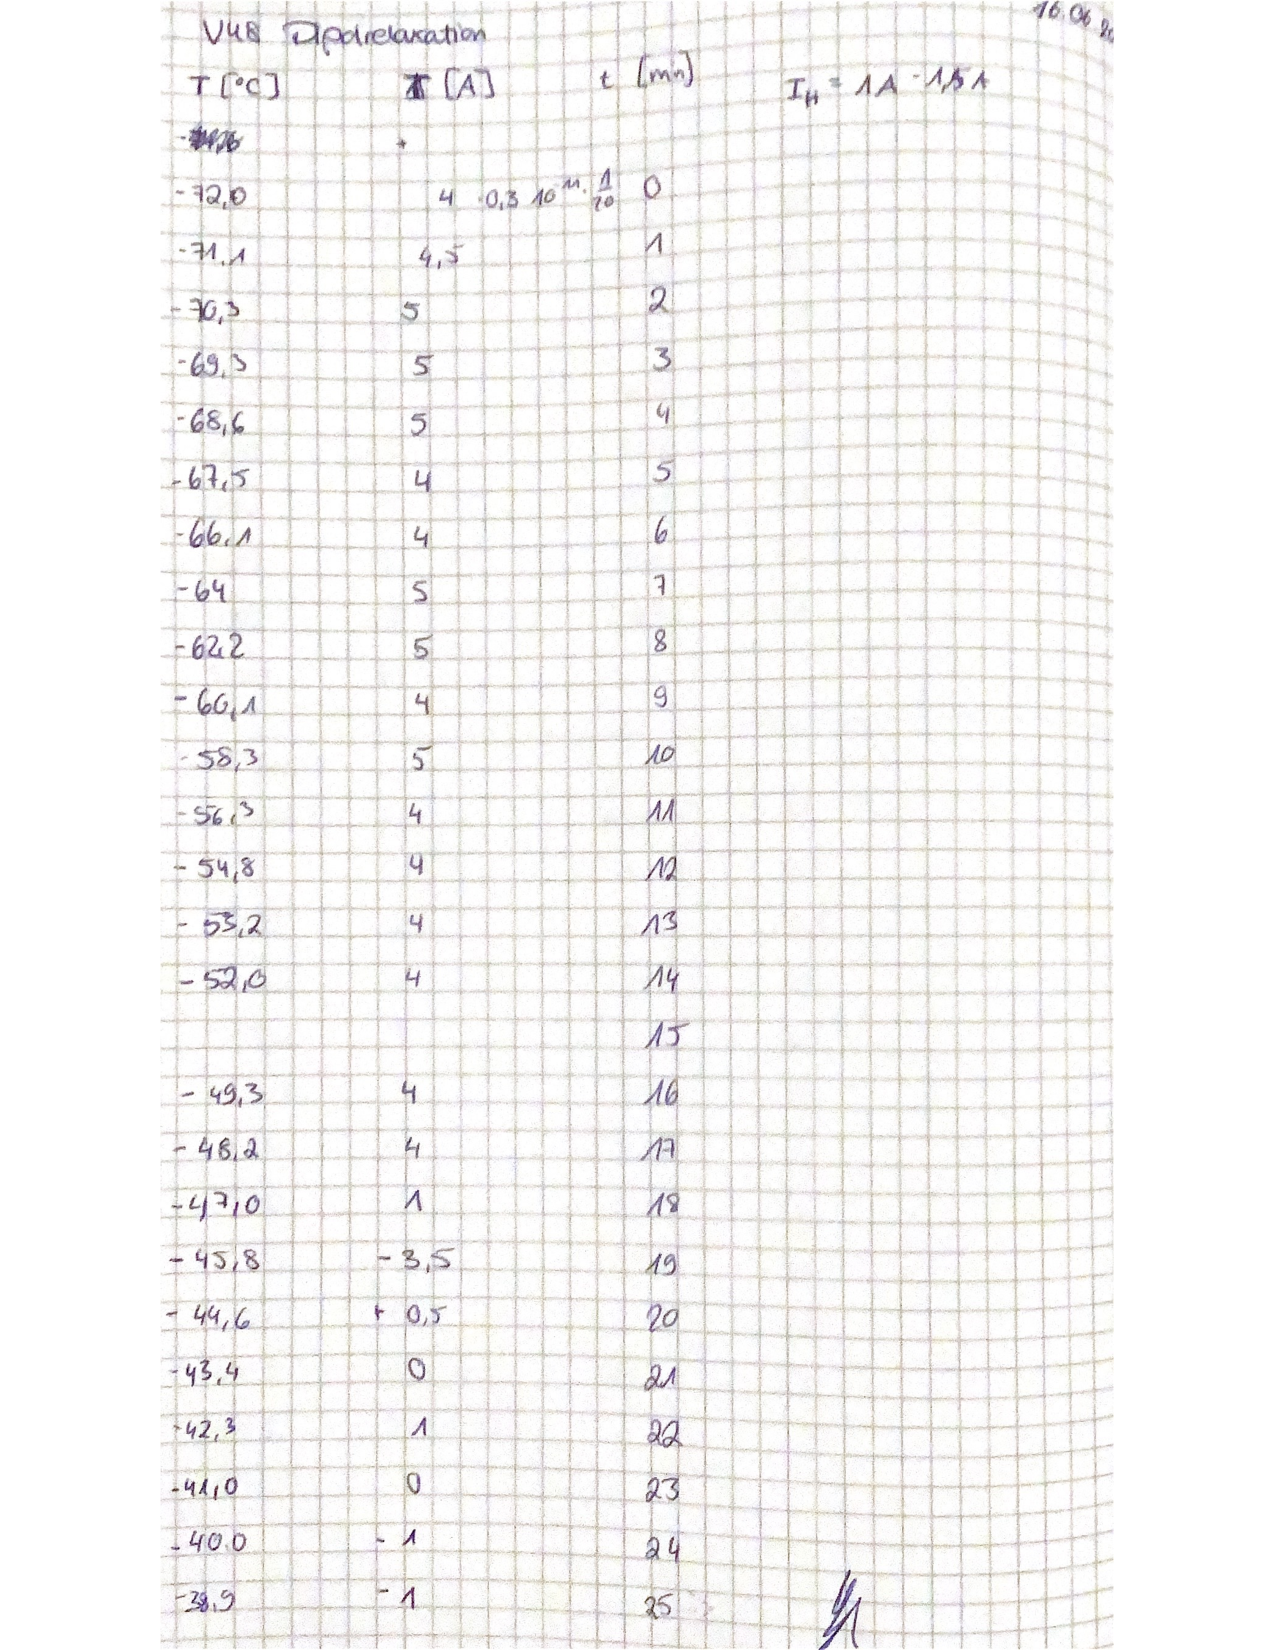
\includegraphics[width=\textwidth]{Bilder/Daten1.pdf}
   \label{fig:Messungen_1}
 \end{figure}
 \begin{figure}[H]
   \centering
   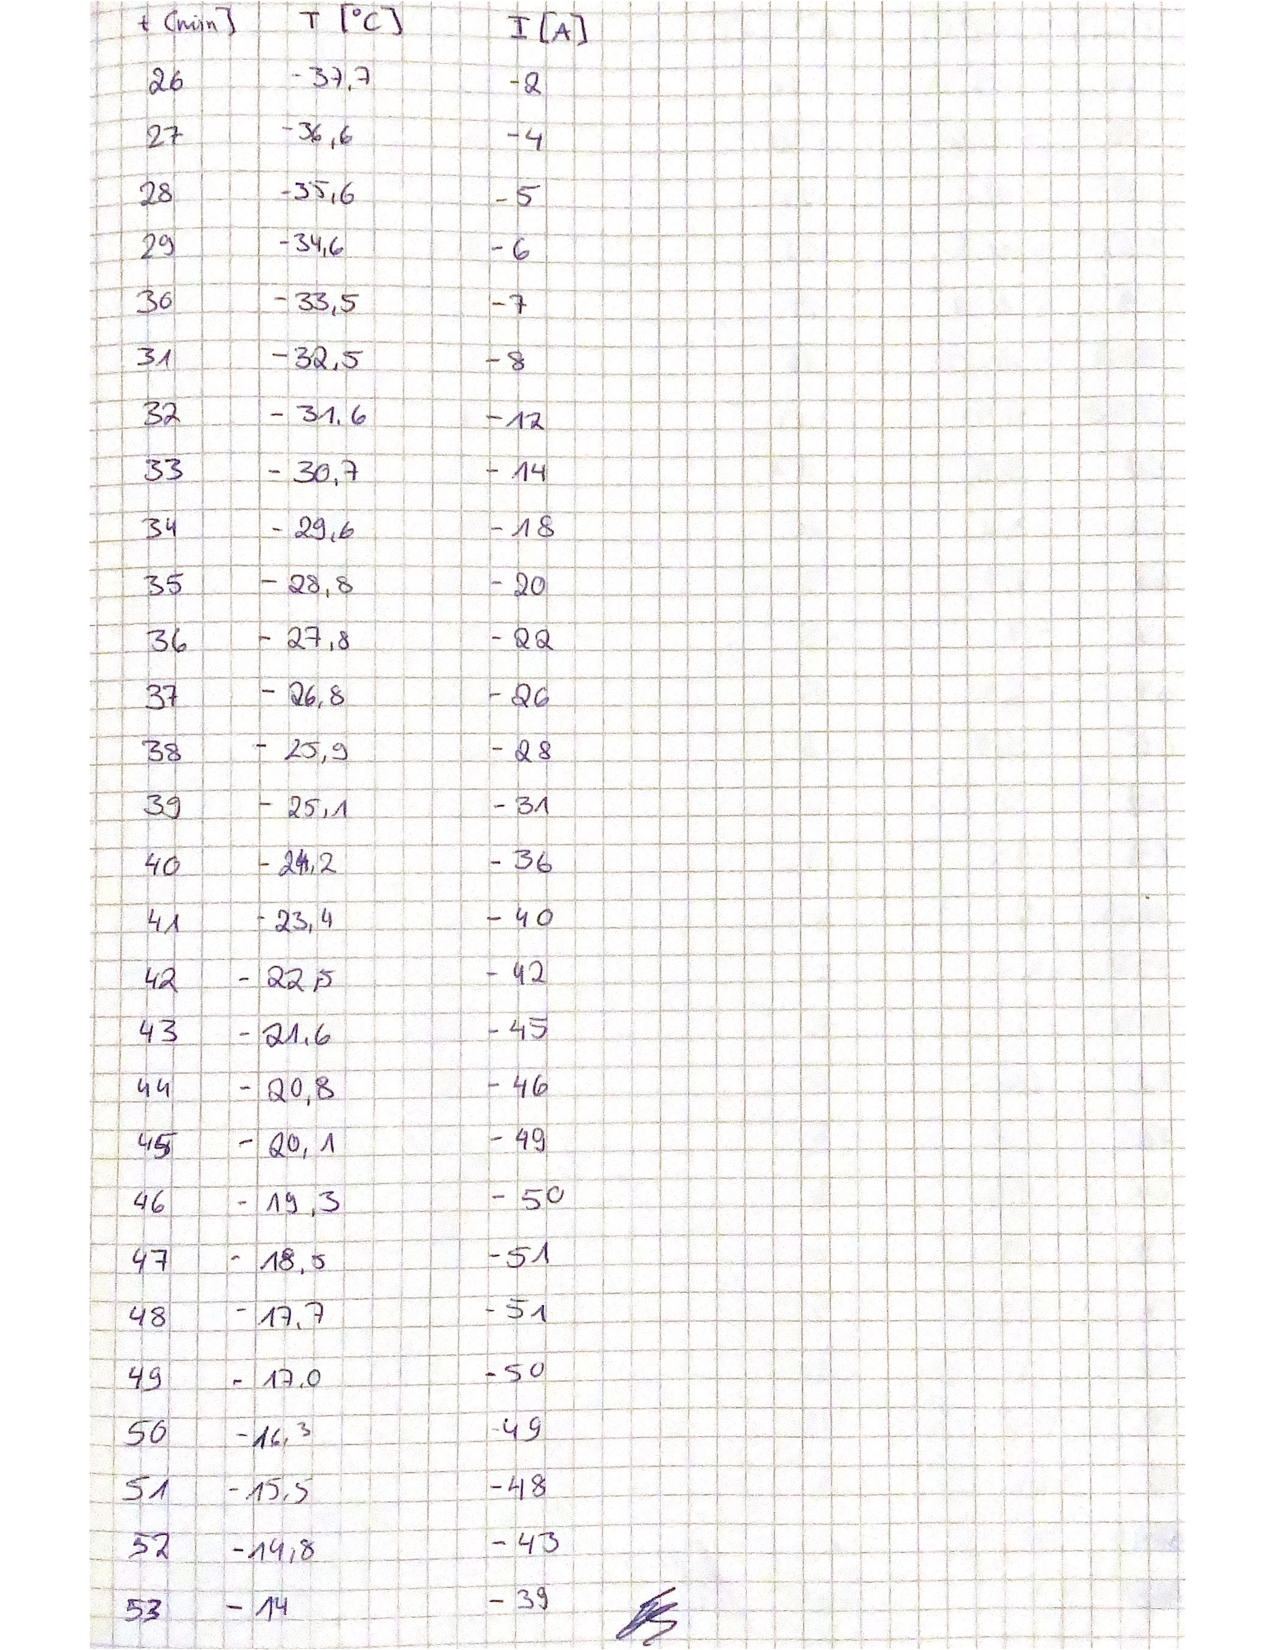
\includegraphics[width=\textwidth]{Bilder/Daten2.pdf}
   \label{fig:Messungen_2}
 \end{figure}
 
 \begin{figure}[H]
   \centering
   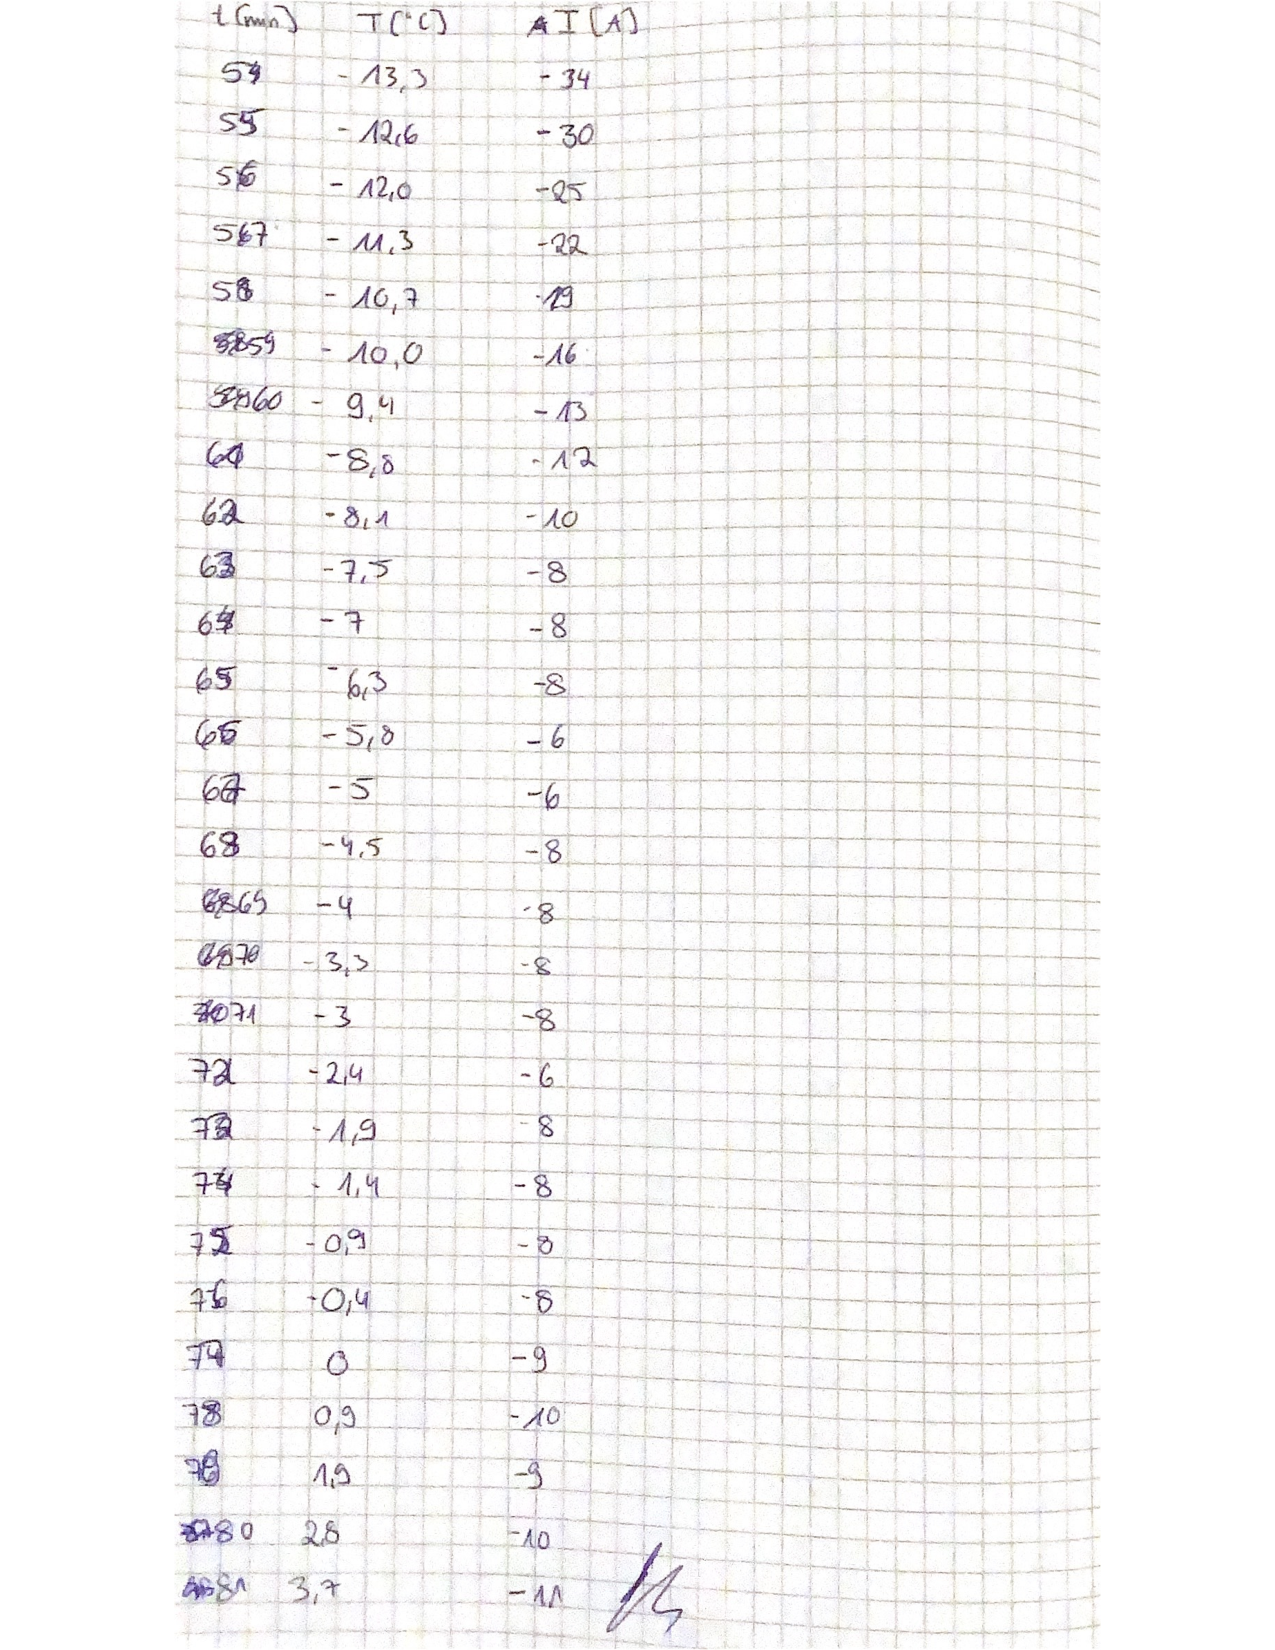
\includegraphics[width=\textwidth]{Bilder/Daten3.pdf}
   \label{fig:Messungen_3}
 \end{figure}
 \begin{figure}[H]
   \centering
   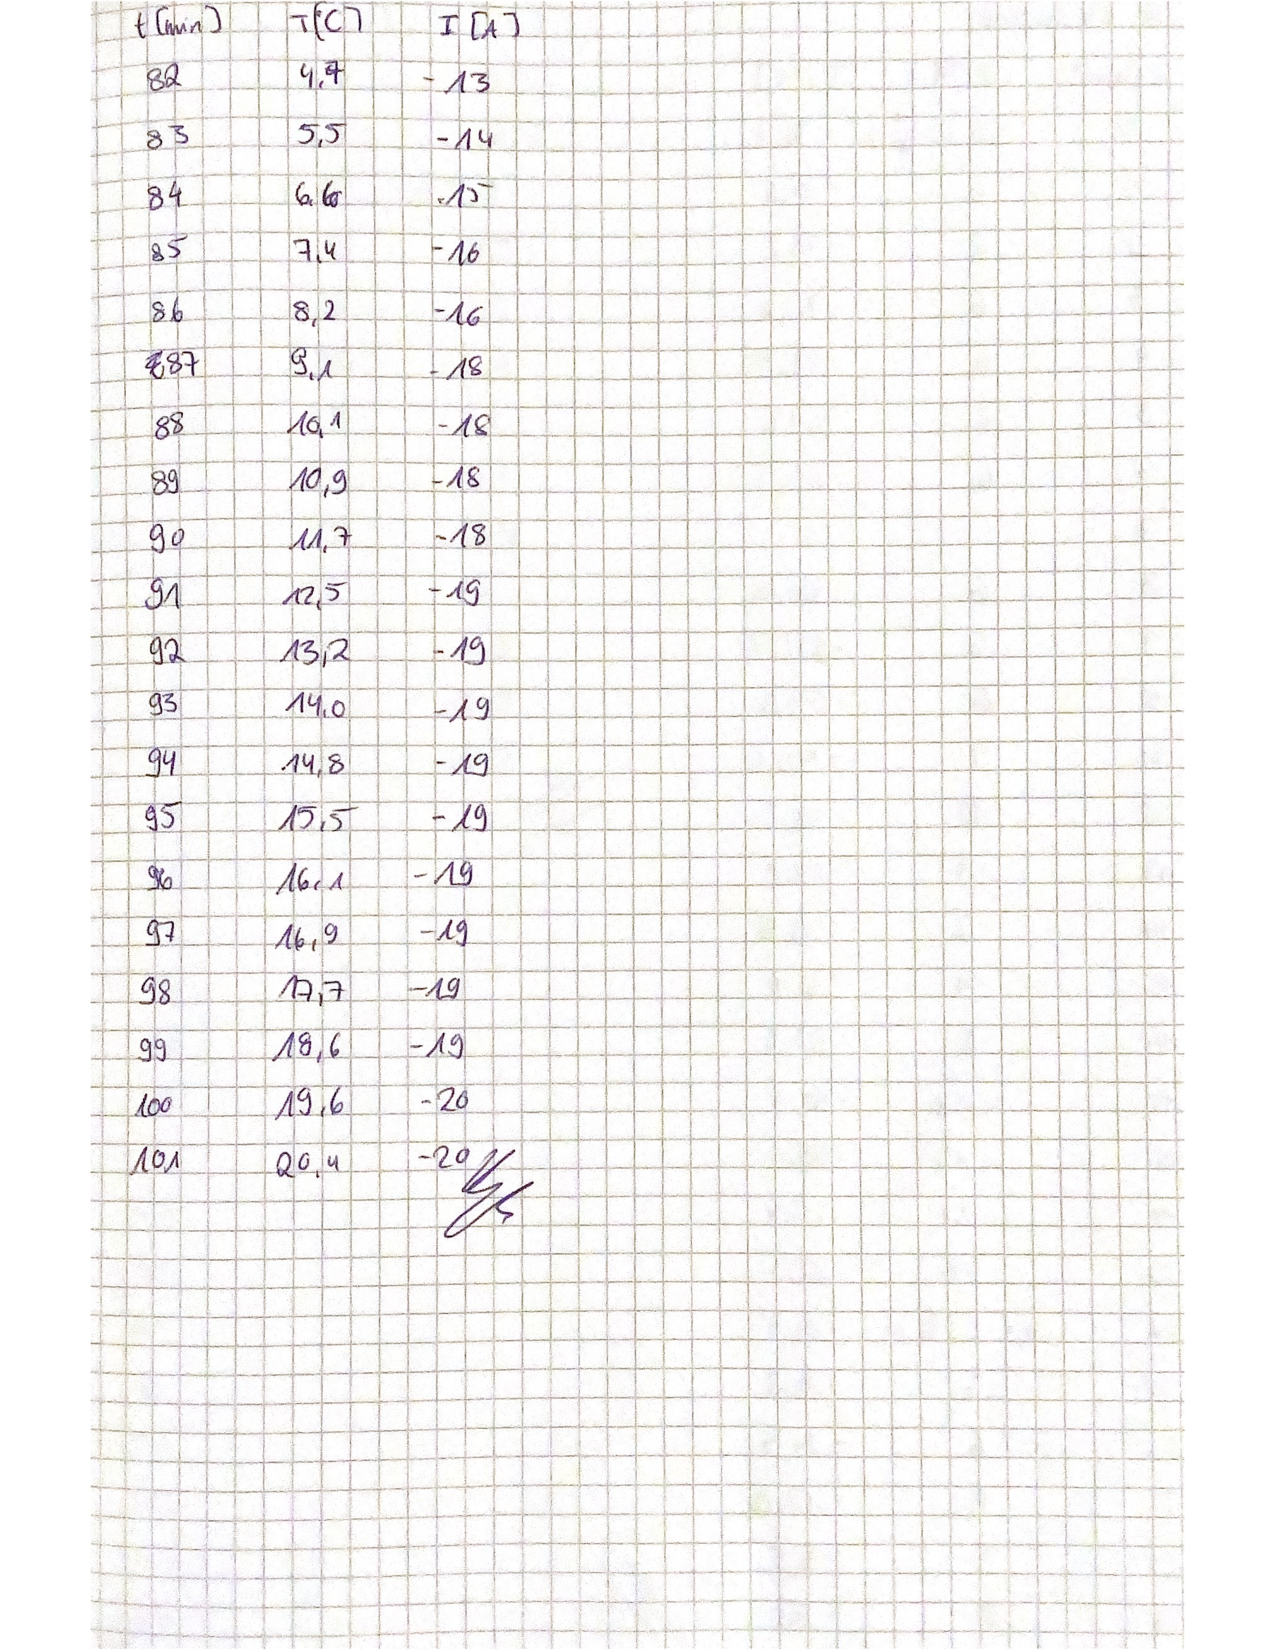
\includegraphics[width=\textwidth]{Bilder/Daten4.pdf}
   \label{fig:Messungen_4}
 \end{figure}
 \begin{figure}[H]
   \centering
   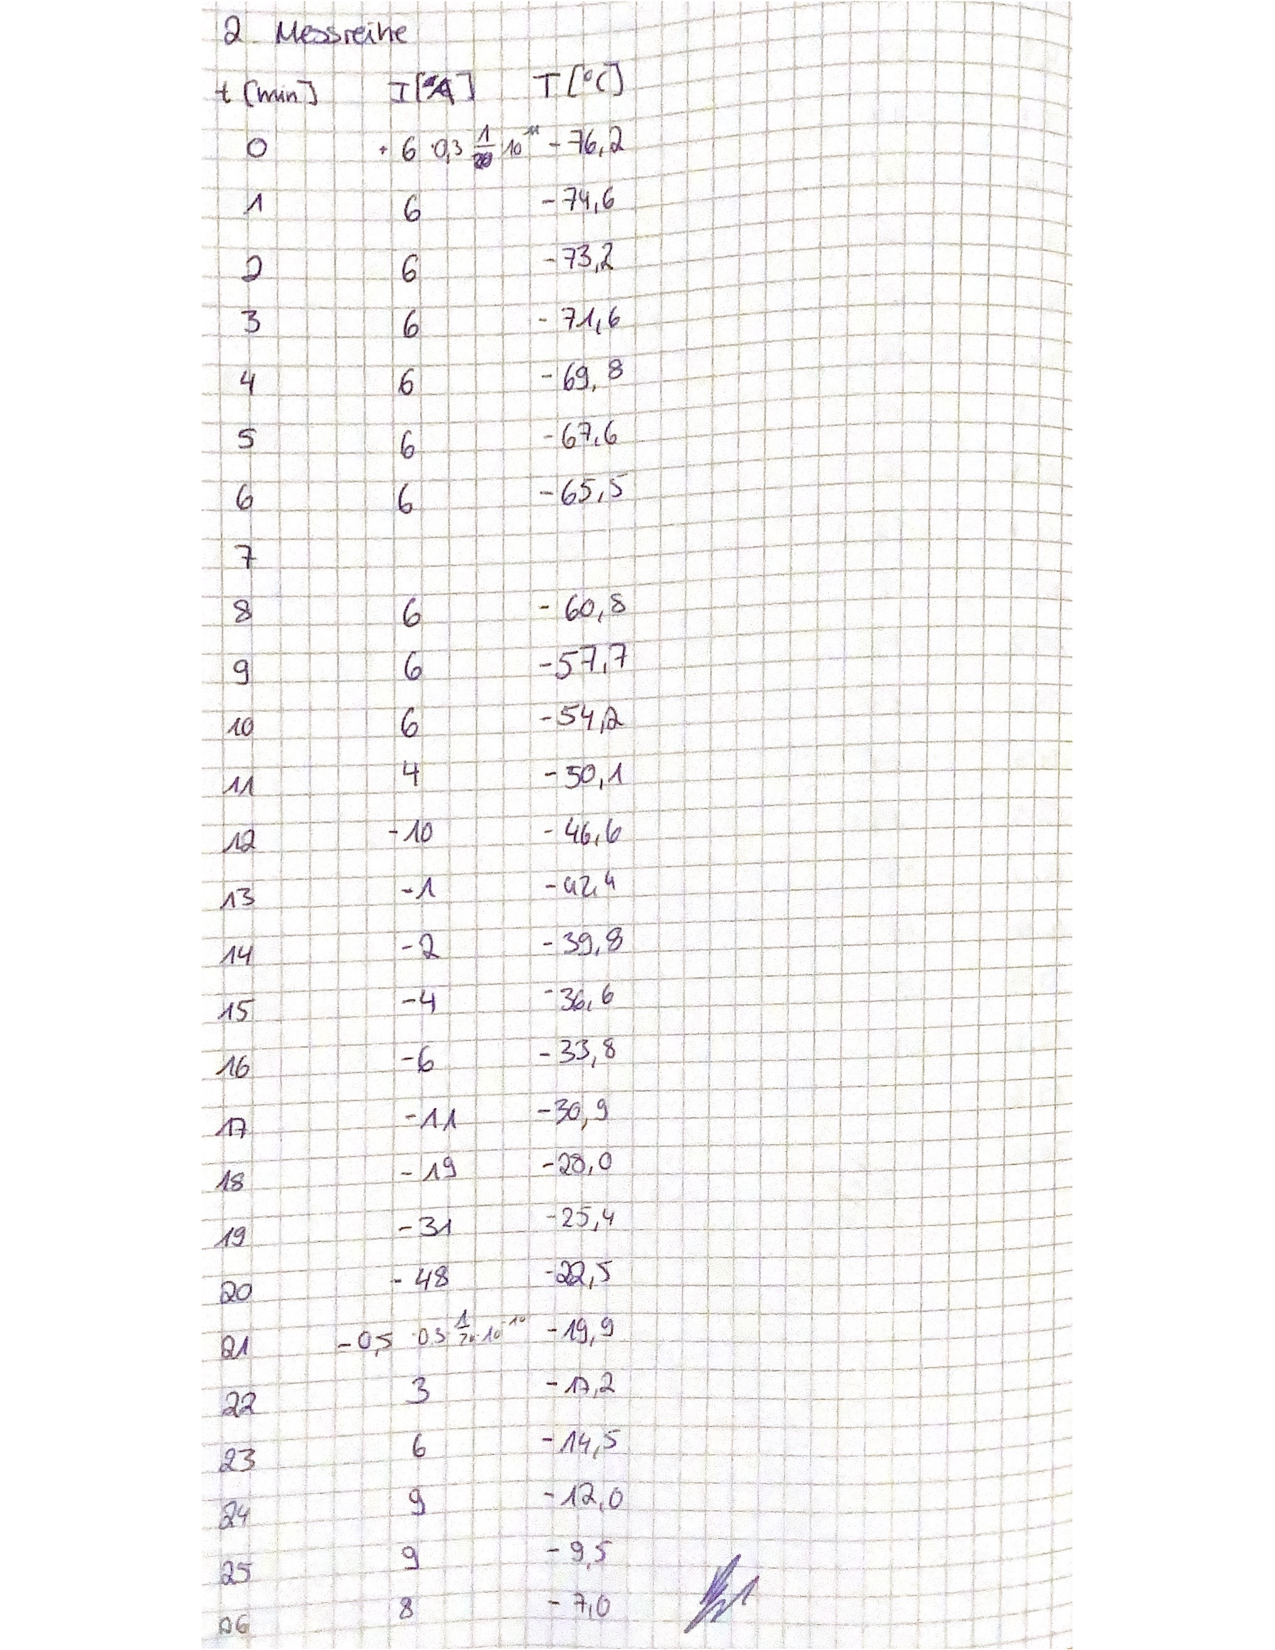
\includegraphics[width=\textwidth]{Bilder/Daten5.pdf}
   \label{fig:Messungen_5}
 \end{figure}
 
 \begin{figure}[H]
   \centering
   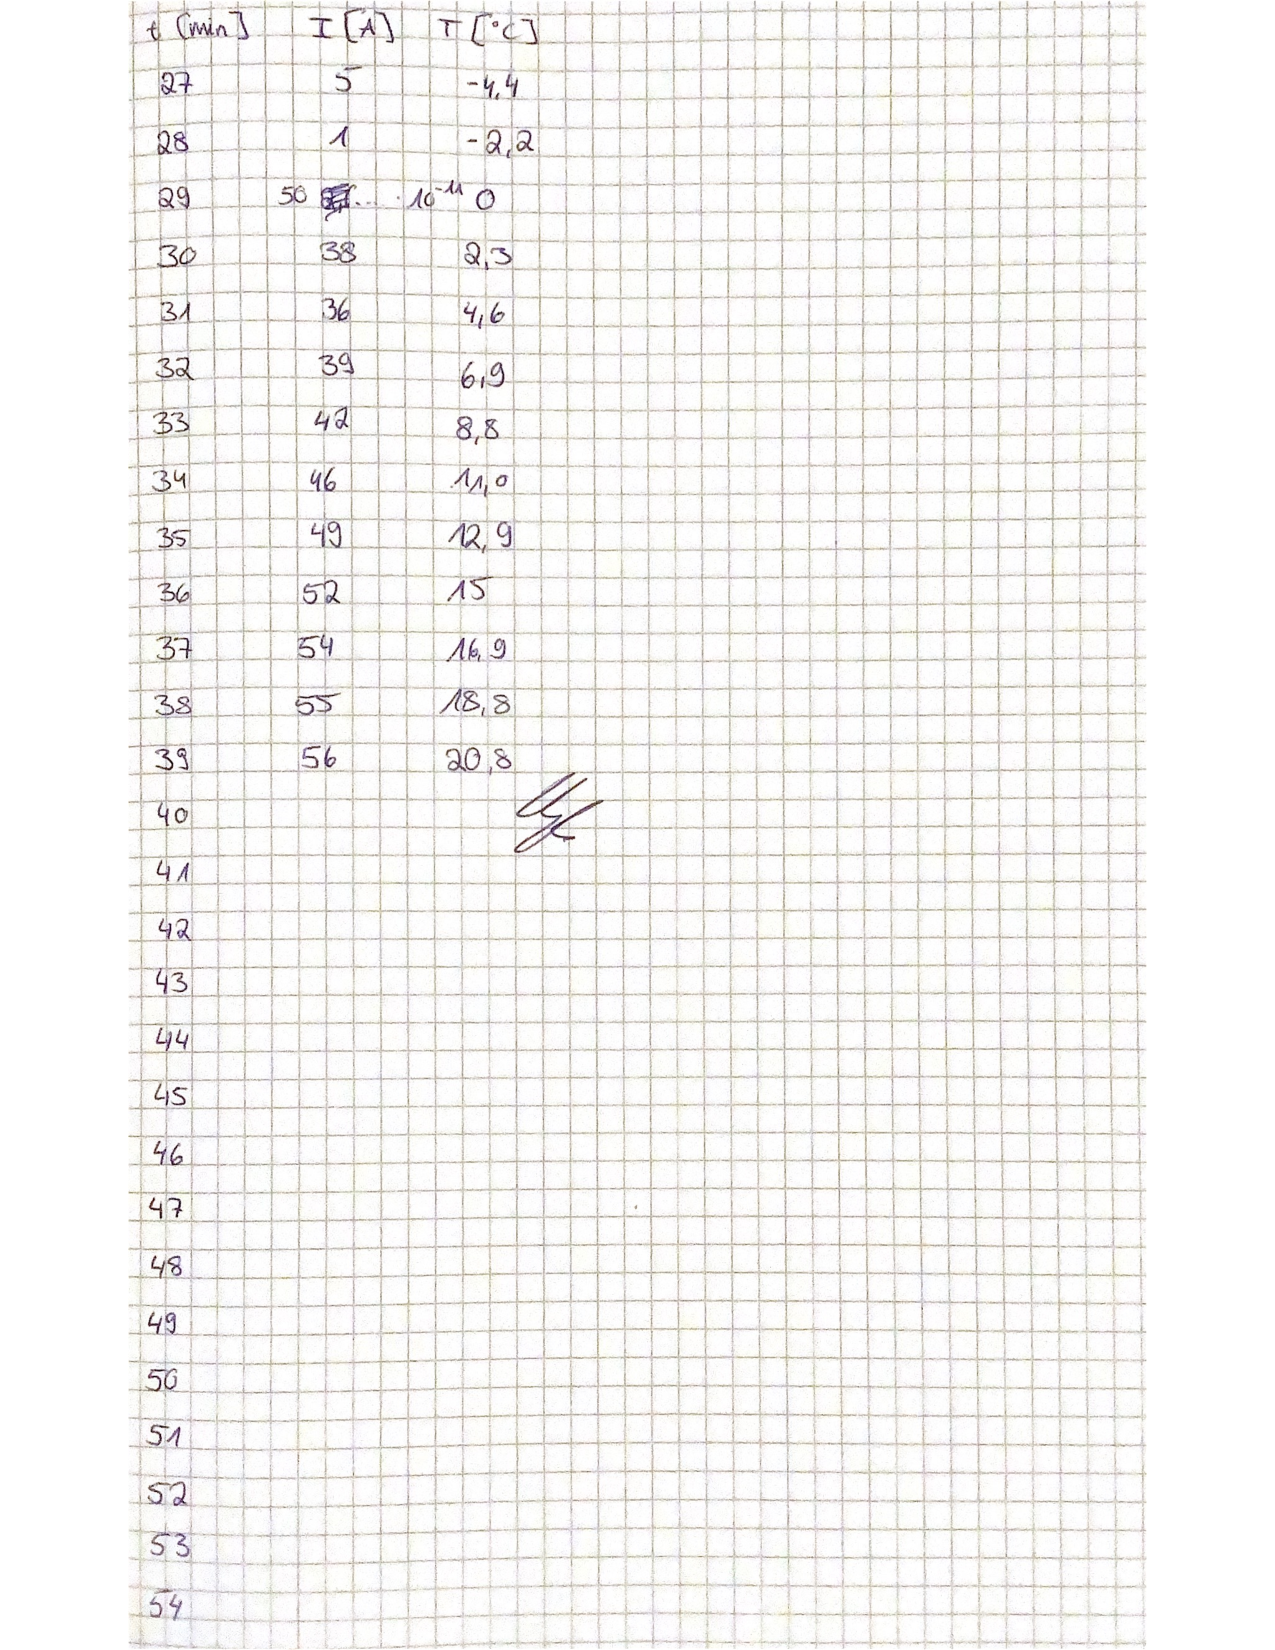
\includegraphics[width=\textwidth]{Bilder/Daten6.pdf}
   \label{fig:Messungen_6}
 \end{figure}

